% !Mode:: "TeX:UTF-8"
%%% Local Variables:
%%% mode: latex
%%% TeX-master: t
%%% End:

% 绪论和国内外现状

\chapter{绪论}
\label{cha:intro}
近些年来,随着人工智能和大数据技术的兴起和应用,知识库逐渐变得流行起来,越来越多的商业机构和科研院所开始构建大规模知识库,如Google Knowledge Graph\cite{Dong},NELL\cite{NELL-aaai15},YAGO\cite{Suchanek:2007:YCS:1242572.1242667},
Freebase\cite{Bollacker:2008:FCC:1376616.1376746},DBpedia\cite{Bizer:2009:DCP:1640541.1640848}等。
这些知识库基于自动的信息抽取、半监督学习、专家知识等技术构建,拥有大量的实体、关系和属性信息。
这类知识库可用性的重要指标通过数据完整性、数据精确性和数据质量等进行衡量,
已经有很多基于知识库的系统被用于商业领域,如谷歌搜索引擎\footnote{https://googleblog.blogspot.com/2012/05/introducing-knowledge-graph-things-not.html},
微软的必应搜索\footnote{https://blogs.bing.com/search/2013/03/21/understand-your-world-with-bing/}等。
除此之外,知识库也被用于生物学\cite{Dumontier:2014:BRL:2878453.2878554}、问答系统、个人手机助手等领域。

当前知识库相关的学术研究主要分为三个方面:(1)知识库的构建,各种基于网络的、通用的、领域内的知识库构建。
(2)关系机器学习,基于已经构建好的知识库进行关系预测,知识库补全推理等。(3)知识库应用系统。如基于知识库的问答系统,
基于知识库的信息检索系统,生物金融等领域的知识库构建等。

\section{知识库构建}
数据完整性、数据精确性和数据质量是构建知识库的重要指标,
通常知识库可以由三元组组成。知识库的构建可以有多种方法:
(1)通过机器学习和自然语言处理技术自动抽取三元组\cite{Weikum2010FromIT}进行构建。
(2)半自动抽取的方法,通过从维基百科等网站的infobox基于规则模式抽取三元组。
(3)基于协同创作\cite{Vrandecic2014WikidataAF}的方法,通过众包的形式系统创建知识库。
(4)基于专家知识构建的领域内知识图谱,这些领域知识图谱有较高的专业性。

图\ref{kb}是一个简单的知识库例子,常见的知识库可以用这类属性图进行表示。
知识库三元组分为关系型三元组和属性事实三元组。关系三元组典型的例子如:北京师范大学,位于,北京。其中“北京师范大学”和“北京”是实体,
表示现实中存在实实在在的事物、人地点等,“位于”是描述实体对之间的关系。属性事实三元组如:北京,人口,2150万。
其中“北京”是实体,“2150万”是描述实体属性的属性值,“人口”是北京这类实体具有的一种属性。

\begin{figure}[H]
\begin{center}
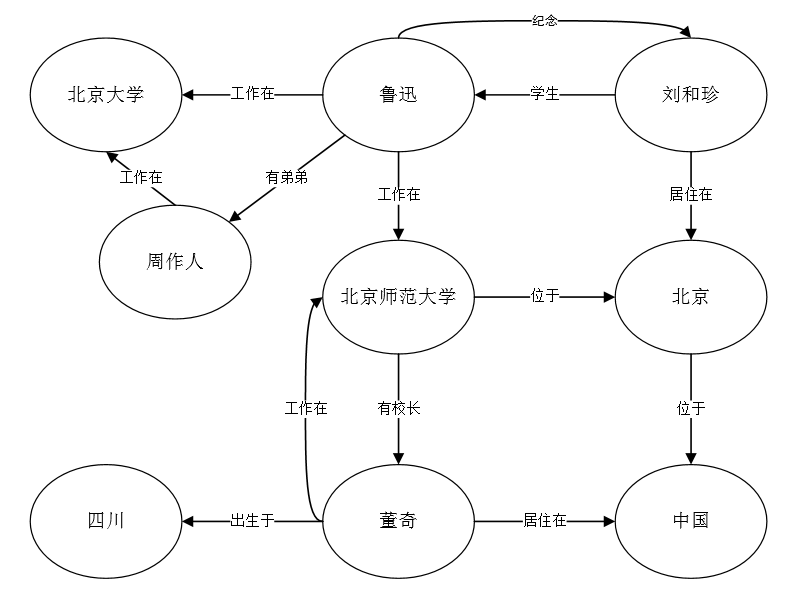
\includegraphics [width=0.5\textwidth]{kb.png}
\caption{一个知识库例子}
\label{kb}
\end{center}
\end{figure}

\section{知识库应用}
知识库最广泛的应用是谷歌和微软等商业公司的信息检索系统。2014年谷歌提出的知识图谱\cite{Dong2014KnowledgeVA}就是
结合FreeBase和互联网数据进行信息抽取,知识整合后的著名系统,谷歌也在其博客上讲述了如何将知识库应用在实际的检索中,
微软的Satori也是一个类似的知识库系统,被必应搜索广泛应用。其他搜索公司如百度、搜狗等公司都在知识库构建和信息检索领域有各自的应用。

基于知识库的问答系统也有广泛的发展。2000年就有人提出基于知识的问答系统\cite{HERMJAKOB2000KnowledgeBasedQA}。
有很多方法基于知识库进行表示学习\cite{Yang2014JointRE},然后构建相关的知识库问答系统。还有一些基于标签语义解析的方法,
构建知识库问答系统\cite{Yih2016TheVO}。
一些论文\cite{Yu2017ImprovedNR}研究结合深度学习、关系抽取和问答系统,从而获得更好的知识库问答效果。
一些论文\cite{KeySun2016OpenKB}研究基于开放的知识库构建开放领域的问答系统,期望能基于百科知识进行问答系统构建。
也有基于知识库的系统通过结合智能计算\cite{Pandey2009KnowledgeAI},在医疗诊断领域获得一些突破。
也有一些研究结合了知识库和医疗图像信息\cite{Halpern2014EvaluationOC},对一些医疗疾病进行诊断治疗,期望能获得更好的治疗效果。

\section{知识库补全和推理} 
虽然许多知识库的规模很大,但他们仍然是不完备的,如很多人的出生地点并未包含在知识库中,
一些演员是否出演过某些电影也是未知的。为了解决这个问题,很多知识库补全的方法被提出来,
这类方法基于知识库中已有的三元组预测新的三元组,如果将现有的知识库数据看做是多种关系构成的图,
图的顶点是实体,图的边是实体对之间的关系,知识图谱补全可以看成是图中关系的预测。
很多经典的知识库补全算法被提出,这些算法可以分为两类:基于逻辑符号推理的补全算法和基于表示学习的补全算法,
有时候也被称为基于图特征和基于隐藏特征的补全算法。

我们研究了常见的YAGO2知识库,发现总共有四百多万实体关系数据被和三百多万属性事实的三元组。
其中的实体关系数据在以往经典的知识库补全算法中被广泛使用,而属性事实数据尽管大量存在,
却在知识库补全系统中并没有得到广泛应用,
同时实体属性数据类型单位差别很大,难以进行统一有效的处理,将这些实体属性特征作为知识库补全的特征也十分困难。
但可以预见在知识库关系预测中,实体属性特征会起着重要的作用,
如何将实体属性三元组有效用于知识库补全是本论文的关键点之一。

此外知识库中的图是稀疏的,每个存在的正例三元组实体对在训练模型中,
可能生成上百组负例三元组实体对,如何解决正负实体对不匹配的问题很关键,在正负实体对比例悬殊时,
关系预测中仅靠逻辑符号推理中的打分模型是不够的,在结果评价中并未考虑候选实体对的顺序对预测结果的影响,
也不关注候选实体的秩序关系,这也是知识库补全算法中需要解决的难点之一。

针对现有知识库补全技术不足,本发明将知识库中的关系路径特征和实体属性特征相结合,构建了一个更准确的知识库补全模型。首先,基于 经典的路径排序模型抽取了关系路径特征;其次通过结合实体属性特征和关系路径特征,构建逻辑回归模型进行关系预测,从而进行知识库补全。
除此之外,本研究提供一种基于学习排序算法的知识库补全技术,
我们通过计算候选头实体和尾实体在关系预测中的位置排序,通过优化排序损失函数MAP来保证训练误差最小,
从而获得最优的关系预测结果,并选择合适的模型评价指标来评估改进我们的预测结果。

\chapter{国内外研究现状}
\label{cha:relatedwork}
当前知识库补全方法主要有两种方法:基于基于表示学习的知识库补全和基于符号逻辑的知识库补全。
基于表示学习的方法是通过学习实体和关系的低维度向量表示,
用向量的相似度计算预测实体之间的关系。常见的表示学习方法有TransE\cite{NIPS2013_5071}、TransH\cite{Wang2014KnowledgeGE}、
TransR\cite{Huang2017ImprovedKB}等,也有基于矩阵张量分解的表示学习方法如RESCAL\cite{Nickel2011}等。
基于符号逻辑的方法主要包括AMIE\cite{Galrraga2013AMIEAR}、PRA\cite{Lao2010}和SFE\cite{Gardner2015}等;其中,AMIE方法通过从知识库中挖掘关联规则进行知识库补全,
PRA方法基于连接实体的关系路径来预测它们之间的关系,SFE在PRA框架的基础上,
抽取更多隐藏的关系路径特征进行模型预测。

\section{基于表示学习的知识库补全}
\label{cha:presentation}
基于学习表示的知识库补全技术是近年来的研究热点之一。近年来获得了极大的关注热度。
这类知识库补全技术通过不同的目标函数,希望能学习到知识库中实体和关系的低维度向量表示。
这些实体的向量维度通常是50-300维度之间,将高维度稀疏的图数据张量,学习获得低维度的连续向量表示。
获得实体和关系的向量表示后,可以通过向量之间余弦距离计算实体-关系-实体相似度。

\subsection{RESCAL}
RESCAL是2011年在ICML上发表的一篇基于协同学习解决多关系知识库补全问题的方法。
将实体-关系-实体构建三维的张量矩阵。RESCAL基于潜藏模型,提供了一种有效的表示学习方法。
和其他表示学习模型不同,RESCAL这类模型更多借鉴推荐系统中张量分解算法,训练学习实体和关系的向量表示。
详细来说,RESCAL基于R阶的分解模型,$\chi_k$被分解为:
$$\chi_k \approx AR_{k}A^T, k =1...m$$
其中A表示一个$n\times r$的矩阵,表示n个实体和r种关系组成矩阵,$R_{k}$是一个$r\times r$的矩阵。
则只需要最小化函数:
$$\min \limits_{A,R_k} f(A,R_k)+g(A,R_k)$$
其中$f(A,R_k)$是度量$\chi_k$和$AR_{k}A^T$距离的函数。
$g(A,R_k)$是$A,R_k$的复杂度惩罚项。通过梯度下降等学习算法可以计算获得模型的参数。

其他类似进行知识库补全的方法还有张量分解机算法\cite{Rendle2010FactorizationM},
基于隐藏变量的张量分解机算法\cite{Rendle2012FactorizationMW},结构化的低维表示\cite{2009EmbeddingLS}、无结构化的低维表示等。
基于张量分解模型和推荐系统等领域的协同过滤算法相似,都是从矩阵补全角度学习向量模型。
不同的是在知识库中,矩阵其实是由实体-关系-实体组成的三维张量,而推荐系统中的用户-商品矩阵是二维向量。
一些实验\cite{Dong2014}表明在稀疏的知识库图中,使用张量分解模型有较好的预测效果。

\subsection{TransE}
TransE是2013年谷歌发表在NIPS上的一篇论文,研究考虑如何将知识库中的多种不同的关系、实体,
学习获得它们的低维向量表示,期望能获得$h+r\approx t$效果,其中h和t分别是头实体和尾实体
学习到的低维向量,r是头实体和尾实体之间的关系向量表示。TransE模型定义了间隔损失函数:
$$L=\sum_{(h,r,t)\in S} \sum_{(h',r,t')\in S'}[\gamma+d(h+r,t)-d(h'+r,t')]_{+}$$

其中$\gamma$是间隔超参数,s是真实存在的知识库,$(h,r,t)$是这个知识库中的三元组
,$s'$是负例三元组组成的知识库实体,$(h',r,t')$表示负例三元组。$d(h+r,t)$表示头实体加上关系向量
和尾实体之间的欧氏距离。通过定义间隔损失函数,TransE期望学习的模型能保证正实例对比负实例对距离小,
这样就能保证正实例对比负实例对余弦相似度更高。

其他的算法如TransH和TransR都是基于TransE模型的基础上,通过学习更准确有效的损失函数来获得低维度向量表示。
TransH考虑一些关系中的映射属性知识,如一对一、一对多、多对多关系等,训练学习这些关系的低维度向量表示。
TransR\cite{Lin2015LearningEA}考虑实体和关系的多方面属性,在分割独立的向量空间中学习实体、关系的低维度向量表示。ProjE\cite{Shi2017ProjEEP}
基于神经网络的实体关系投影表示学习。

\section{基于符号逻辑的知识库补全}
\label{cha:symbolic}
基于逻辑符号的知识库补全算法也是多年来知识库补全和知识库推理中的关注热点之一。从90年代昆兰等人提出的规则归纳,
将观察集数据中的知识以规则的形式提炼出来,到近年来热门的基于路径排序算法(PRA)和子图特征抽取(SFE)的知识库推理补全。这类进行知识库补全的算法
多是利用符号逻辑,统计发现知识库图数据结构中存在的规则或规律,从而进行知识库补全预测。

\subsection{规则挖掘}
规则挖掘基于训练集知识库中的数据,通过挖掘知识库中隐藏的关联规则,进行知识发现和知识库补全。早期昆兰等人
提出了一阶逻辑推理的算法FOIL\cite{Quinlan1993FOILAM},通过学习知识库中的例子来构建霍顿子句。如:
$$MotherOf(A,C)\land MarriedTo(A,B)\Rightarrow FatherOf(B,C)$$
就是一个典型的一阶逻辑推理。FOCL\cite{PAZZANI1991DetectingAC}等算法也是基于一阶逻辑推理构建的知识库搜索算法。
近年来随着互联网的快速发展,Schoenmackers\cite{Schoenmackers:2010}等人也将一阶逻辑逻辑推理用于互联网文本中。
其他规则挖掘的典型算法包括AMIE\cite{Galarraga2013},AMIE受关联规则启发,基于开放世界假设,在一阶逻辑推理的基础上,
能更快更高效的处理大规模的知识库数据,作者此后对AMIE算法进行改进获得AMIE+\cite{Galrraga2015FastRM},这些算法在
YAGO知识库中获得了很好的效果。RDF2Rules\cite{Wang2015RDF2RulesLR}等算法也是基于逻辑推理,构建频繁的谓词圈,
获得了更加高效和准确的逻辑推理算法。

\subsection{路径排序算法}
路径排序算法\cite{Lao2010}是2010年,劳逆等人提出的知识库补全算法。在传统的一阶逻辑推理的基础上,
路径排序算法基于随机游走,在由知识库构成的图数据中查找更多、更长的有效的路径进行知识库推理,
和规则学习方法不同,路径排序算法在抽取图中的关系路径后,构建了分类学习器,通过分类器学习不同关系路径的权重。
利用每种关系下三元组的不同关系路径权重,来进行新关系事实的预测,从而构建了新的知识库补全算法。此外,作者还构建了基于反向
的随机游走图搜索算法\cite{Lao2015LearningRF},进一步提升路径排序算法在知识库补全中的效果。考虑给定一个知识库关系$r_i$,
我们抽取所有具有这种关系的实体对构成集合:
$$R_i=\{{(h_{ij},t_{ij}),(h_{ij},r_i,t_{ij})\in KB}\}$$

随机游走查找路径后,我们抽取所有连接实体对$(h_{ij},t_{ij})$的路径类型$p_i$构成分类特征:
$$P_i=\{{p_i|(h_{ij},p_i,t_{ij})\in KB}\}$$

从而我们可以选择合适的分类器模型进行关系路径的训练学习,利用合适的路径类型来进行关系预测,知识库补全。

子图特征抽取\cite{Gardner2015}提供了一种更加简便有效的关系路径计算方法。相比于路径排序算法,子图特征抽取能获得更多的潜藏路径,
在进行关系预测的时候能获得更加显著有效的提升。此外,也有很多算法结合了子图特征抽取和表示学习算法\cite{Gardner2014}进行知识库补全。
一些算法对相似的关系进行聚类,构建多任务的路径排序模型\cite{Wang2016}。


\section{知识库补全假设}
知识库补全系统中,通常需要假定知识库中三元组正负实例对的正确性,或者在何种限制模式生成三元组负例。常用的有三种假设:(1)开放世界假说,(2)
封闭世界假说,(3)局部封闭世界假说。我们给定一个三元组集合$D^+$表示正例:
$$D^+=\{(h,r,t)|(h,t) \in KB\}$$

对于开放世界假说,给定一个知识库中的三元组集合,我们认为这些实际存在三元组是正例三元组,对于在知识库中不存在的三元组,
开放世界假说认为这个三元组是不确定的,可以通过概率大小预测这个三元组的正确性。

对于封闭世界假说,给定一个知识库三元组集合,我们认为只有知识库存在的三元组才是正例三元组。对于知识库中不存在的三元组,
封闭世界假说认为这些三元组是负例三元组。但通常这样会产生正负实例极其不平衡情况,每个知识库中存在三元组都能生成数百例
负例三元组。这些负例三元组组成负例集合$D^-$:
$$D^-=\{(h_j,r,t_i)|(h_i \ne h_j \wedge (h_i,t_i) \in KB)\}$$
$$ \cup \{(h_i,r,t_j)|(t_j \ne t_i \wedge(h_i,t_i) \in KB)\}$$

局部封闭世界假说对封闭世界假说进行了改进。给定一个关系,知识库中这个关系的三元组记为正例三元组,随机在这个关系中
替换头尾实体,生成这个关系下实体集合中错误的实体对,这样就可以大大减少所有负例三元组个数。基于局部封闭世界假设
构建的负例三元组集合$D^-$可以用如下公式表示:
$$D^-=\{(h_{ik},r_i,t_{ij})|(h_{ik} \ne h_{ij} \wedge (h_{ik},t_{ik}) \in KB  \wedge (h_{ij},t_{ij}) \in KB)\}$$
$$ \cup \{(h_{ij},r_i,t_{ik})|(t_{ij} \ne t_{ik} \wedge(h_{ik},t_{ik}) \in KB \wedge(h_{ij},t_{ij}) \in KB)\}$$ 